% !TeX root = ../0_Manuscript.tex

%\section{Introduction \ddc}
%\label{chap:2_goodPractices;sect:intro}
%Body Biasing Injection

\section{\bbi platforms in the state-of-the-art \ddcu}
\label{chap:2_goodPractices;sect:bbiPlatforms}
    \subsection{Initial \bbi platforms \ddcu}
    First introduced in 2012 by P. Maurine et al. \cite{bbiOrigin}, further studied in 2013 by K. Tobick et al. \cite{bbiSecond}, the proposed \bbi platform in both papers is fairly simple, similar to \emfi platforms, composed of:
    \begin{itemize}
        \setlength\itemsep{-0.1em}
        \item A decapped IC, with its backside accessible
        \item An independent voltage pulse generator able to generate positive voltage pulses up to 100 V, with a maximum current of 2 A. The generator is DC-coupled with the load.
        \item A passive custom-made probe, consisting of an SMA connector and a needle soldered to it
        \item A positioning system to place the probe precisely onto the IC's backside
        \item An acquisition system, measuring various voltages
    \end{itemize}
    It is important to remark that the probe is connected through a relatively long interconnection, acting as a transmission line.

    \subsection{C. O'Flynn \bbi platform \ddcu}
    The original platform had stayed identical in the literature \cite{bbiThird}, until C. O'Flynn published in 2020 \cite{bbiColin} practical examples of \bbi attacks on WLCSP integrated circuits.
    In this work, the platform is structured differently.
    There are common elements, such as:
    \begin{itemize}
        \setlength\itemsep{-0.1em}
        \item An IC target with an accessible backside, in that case thanks to the WLCSP
        \item A positioning system
        \item Various acquisition tools
    \end{itemize}
    The structural differences concern the voltage pulse generation.
    Instead of an independent voltage pulse generator, connected to a passive probe through a transmission line, the proposed solution consists in implementing an active probe with a separate pulse trigger generator.
    
\begin{figure}[ht]
    \centering
    \includegraphics[width=0.8\textwidth]{2_goodPractices/figures/colinFigureBBI.png}
    \caption{Schematic extracted from C. O'Flynn \cite{bbiColin}: \bbi injection device proposed by C. O'Flynn \cite{bbiColin}, using a transformer to produce high voltage pulses from a low voltage power supply.}
    \label{fig:colinBBIsonde}
\end{figure}

    Fig. \ref{fig:colinBBIsonde} shows the design extracted from C. O'Flynn work \cite{bbiColin}.
    The transformer allows creating high voltage pulses from a low voltage power supply.
    The transformer is controlled through the transistor Q1.
    Because the output is the secondary of a transformer, it is AC-coupled to the load, thus, no DC current can be transferred to the load.
    The transformer is custom-made and allows for ten times voltage multiplication, therefore enabling 300 V pulses with a 30 V power supply unit (PSU), which is fairly common for a lab PSU.
    The transistor is controller thanks to an external trigger pulse, generated by another piece of equipment on this platform.
    It is on this point that O'Flynn's platform greatly differs from Maurine's initial platform.

    The pulse generator used in this paper is a ChipWhisperer-Lite, an open-source tool created by NewAE Technology Inc.
    This tool can perform various tasks, such as pulse generation (as it is currently done), analog signals capture, or clock generation, enabling clock glitch fault injection.
    In addition to that, it can act as a simultaneous capture and target board, which is of great use in a \bbi context.

    \subsection{Commercial platforms \ddcnew}
    In addition to documented research \bbi platforms, there are multiple commercially available solutions.
    We are going to address the most noteworthy in the current section.

        \subsubsection{Langer EMV-Technik GmbH \bbi platform \ddcnew}
        
\begin{figure}[ht]
    \centering
    \includegraphics[width=0.2\textwidth]{2_goodPractices/figures/langerBBI.jpg}
    \caption{\bbi probe proposed by the company Langer EMV-Technik GmbH.}
    \label{fig:langerBBI}
\end{figure}
        The German society "Langer EMV-Technik GmbH" proposes a ready-to-use \bbi platform.
        It is composed of two main hardware components:
        \begin{itemize}
            \setlength\itemsep{-0.1em}
            \item A \bbi current pulse generator, illustrated in Fig. \ref{fig:langerBBI}.
            \item A "Burst Power Station", which is the combination of a power supply and a controller allowing to control and monitor every probe sold by the company, with a provided software.
        \end{itemize}
        The core design is similar to the state-of-the-art platform, the main difference being that the system commercialized by Langer contains a current source instead of a voltage source.
        However, in practical operation, it does not represent a significant difference, as one can either perform the \bbi experiments with both electrical sources.
        The probe is specified with the following characteristics:
        \begin{itemize}
            \setlength\itemsep{-0.1em}
            \item A maximum allowable current of 4 A in a 1 \textOmega\xspace load
            \item A rise time inferior to 2 ns
            \item A maximum pulse repetition frequency of 20 kHz
            \item Positive and negative polarities
            \item The possibility to delay the pulse command thanks to their control module
        \end{itemize}
        According to the product's datasheet, containing actual measurements of the probe, the minimal intensity allows injecting at peak approximately 2.4 A in 1 \textOmega\xspace.
        However, contrary to the open-source ChipWhisperer-Lite, there is very little official documentation about their products, thus reducing the available knowledge.

% PAS ENCORE RETOUCHÉ ICI - début
{\color{orange}{NOTRE PLATEFORME APRÈS, structure à revoir.
Body Biasing Injection platforms are constituted of many tools and equipment.
It is quite similar of the one used in \emfi, and is composed of:
\begin{itemize}
    \setlength\itemsep{-0.1em}
    \item A metallic probe (EM probe in \emfi), allowing high electric current and fast pulses
    \item A voltage pulse generator capable of generating very high, short and precise pulses
    \item A 3D positioning table, with a precision under 10 µm to place the probe precisely with correct pressure on the backside
    \item A vibration-proof table to minimize probe jitter due to vibration caused by other equipment or natural vibration
    \item A high precision oscilloscope to measure various physical quantities that might help to practice \bbi
\end{itemize}
Among these tools, most are optional and play a role in improving the flexibility and accuracy of \bbi.
Therefore, we describe in details the probe and the generator as they represent the key equipment when performing \bbi.

\subsection{Probes \ddc}
\label{chap:2_goodPractices;sect:bbiPlatforms;subsect:probes}

%\begin{figure}[H]
%    \centering
%    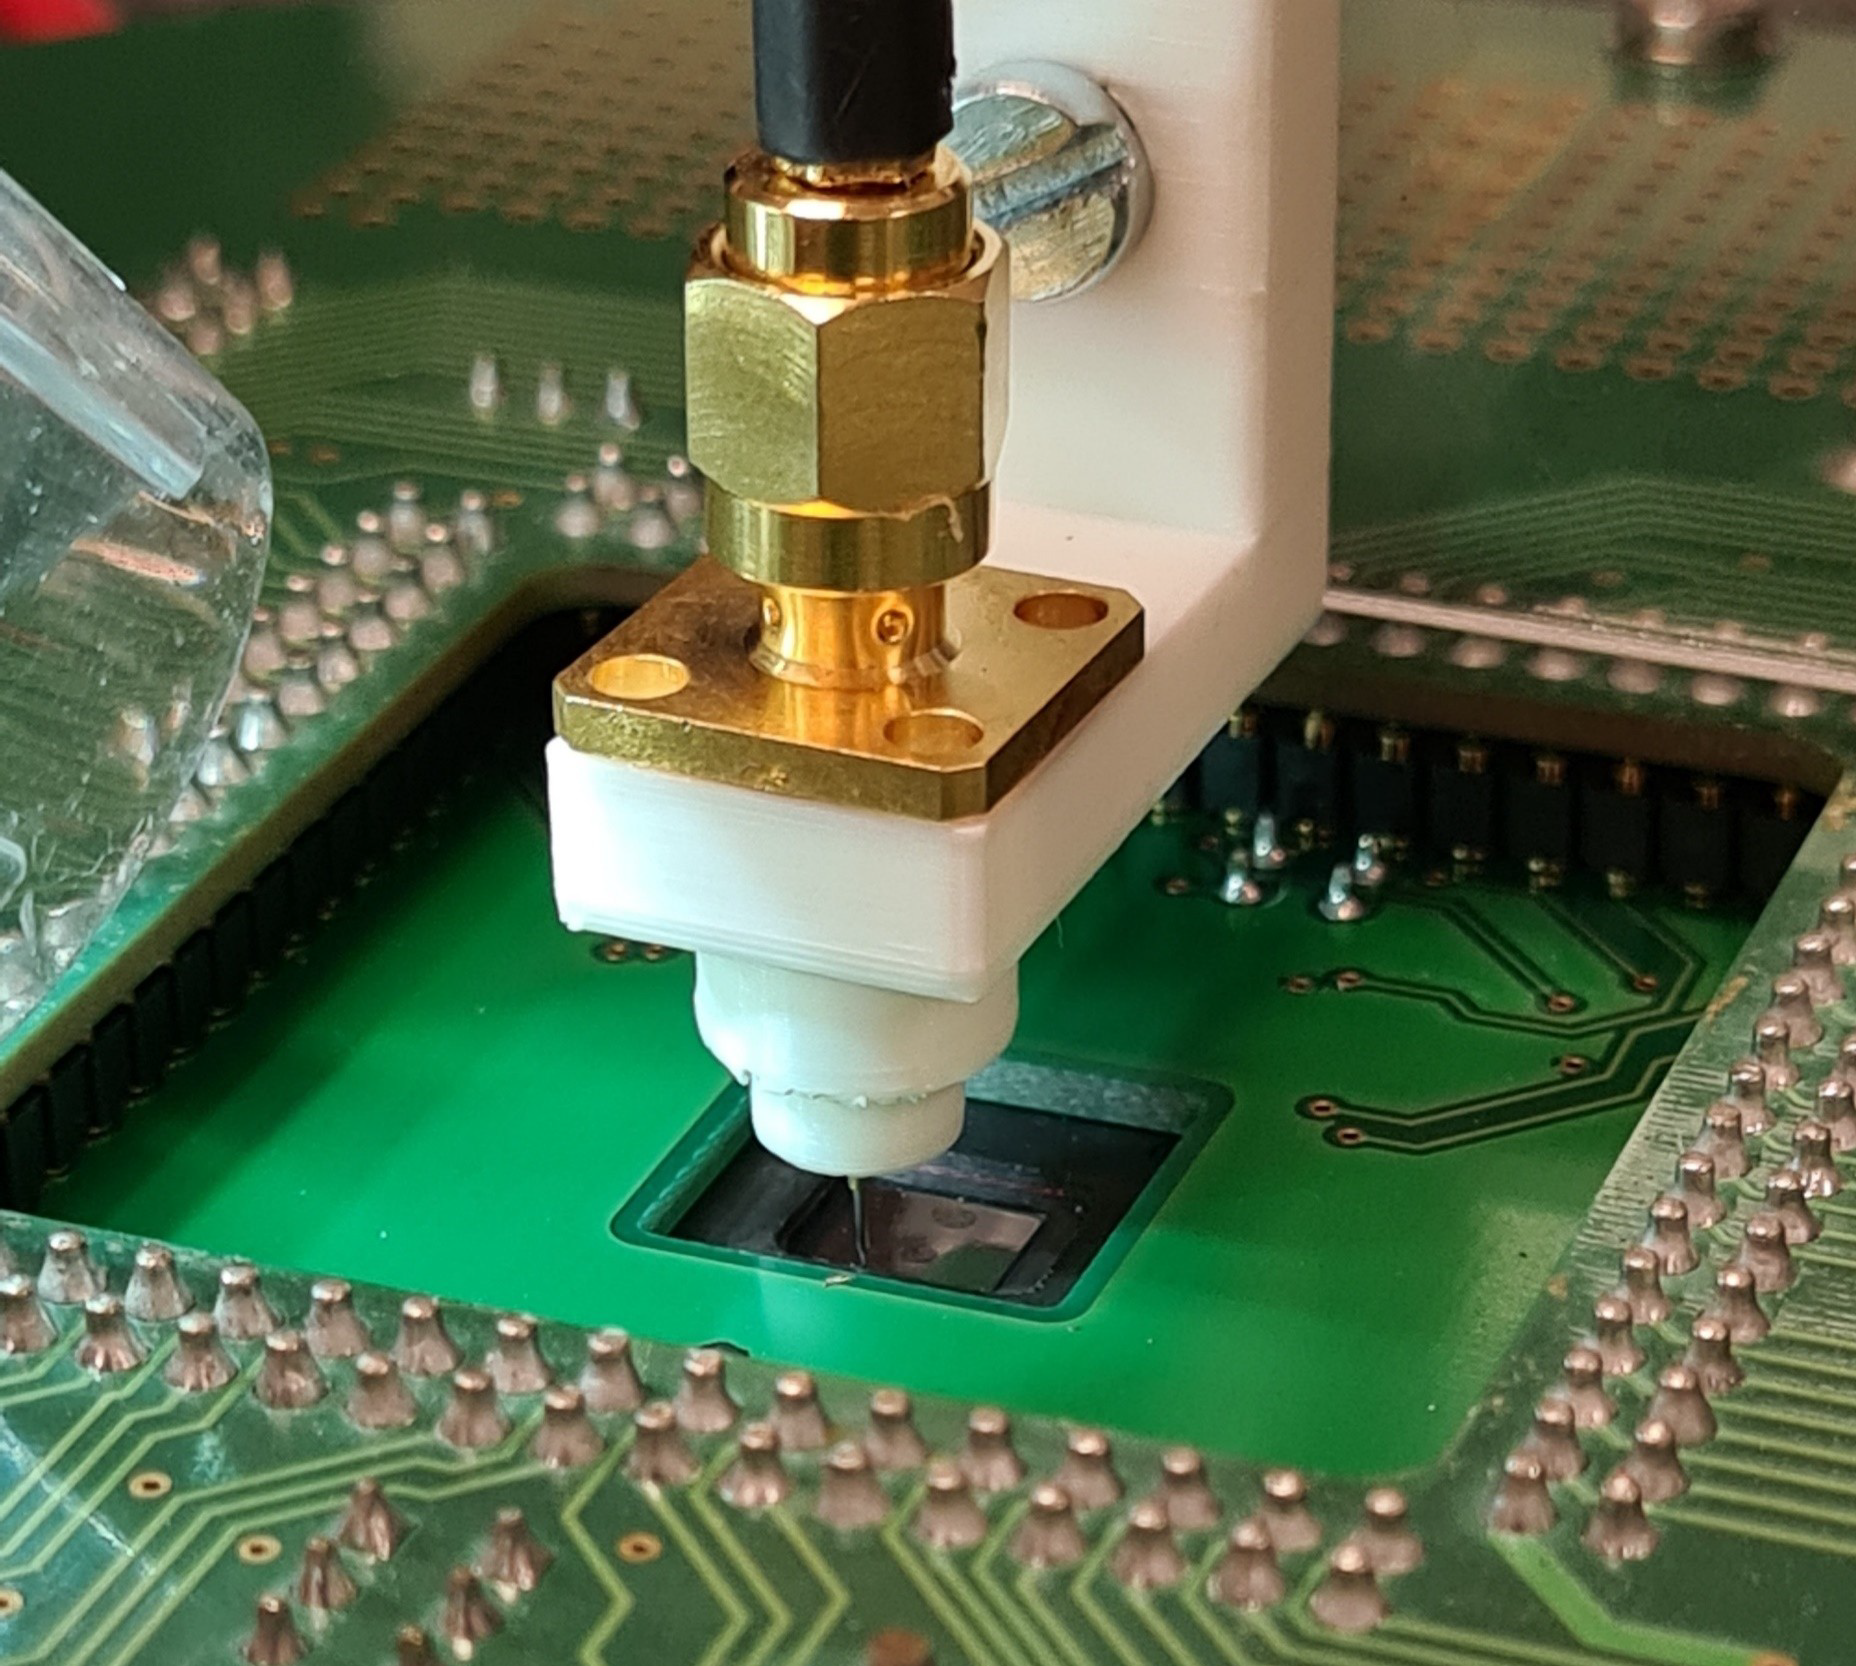
\includegraphics[width=16cm]{2_goodPractices/figures/sondeBBI_loin_raw.png}
%    \caption{BBI metallic probe in mechanical contact with IC target}
%    \label{fig:sondeBBI}
%\end{figure}
%
%\begin{figure}[H]
%    \centering
%    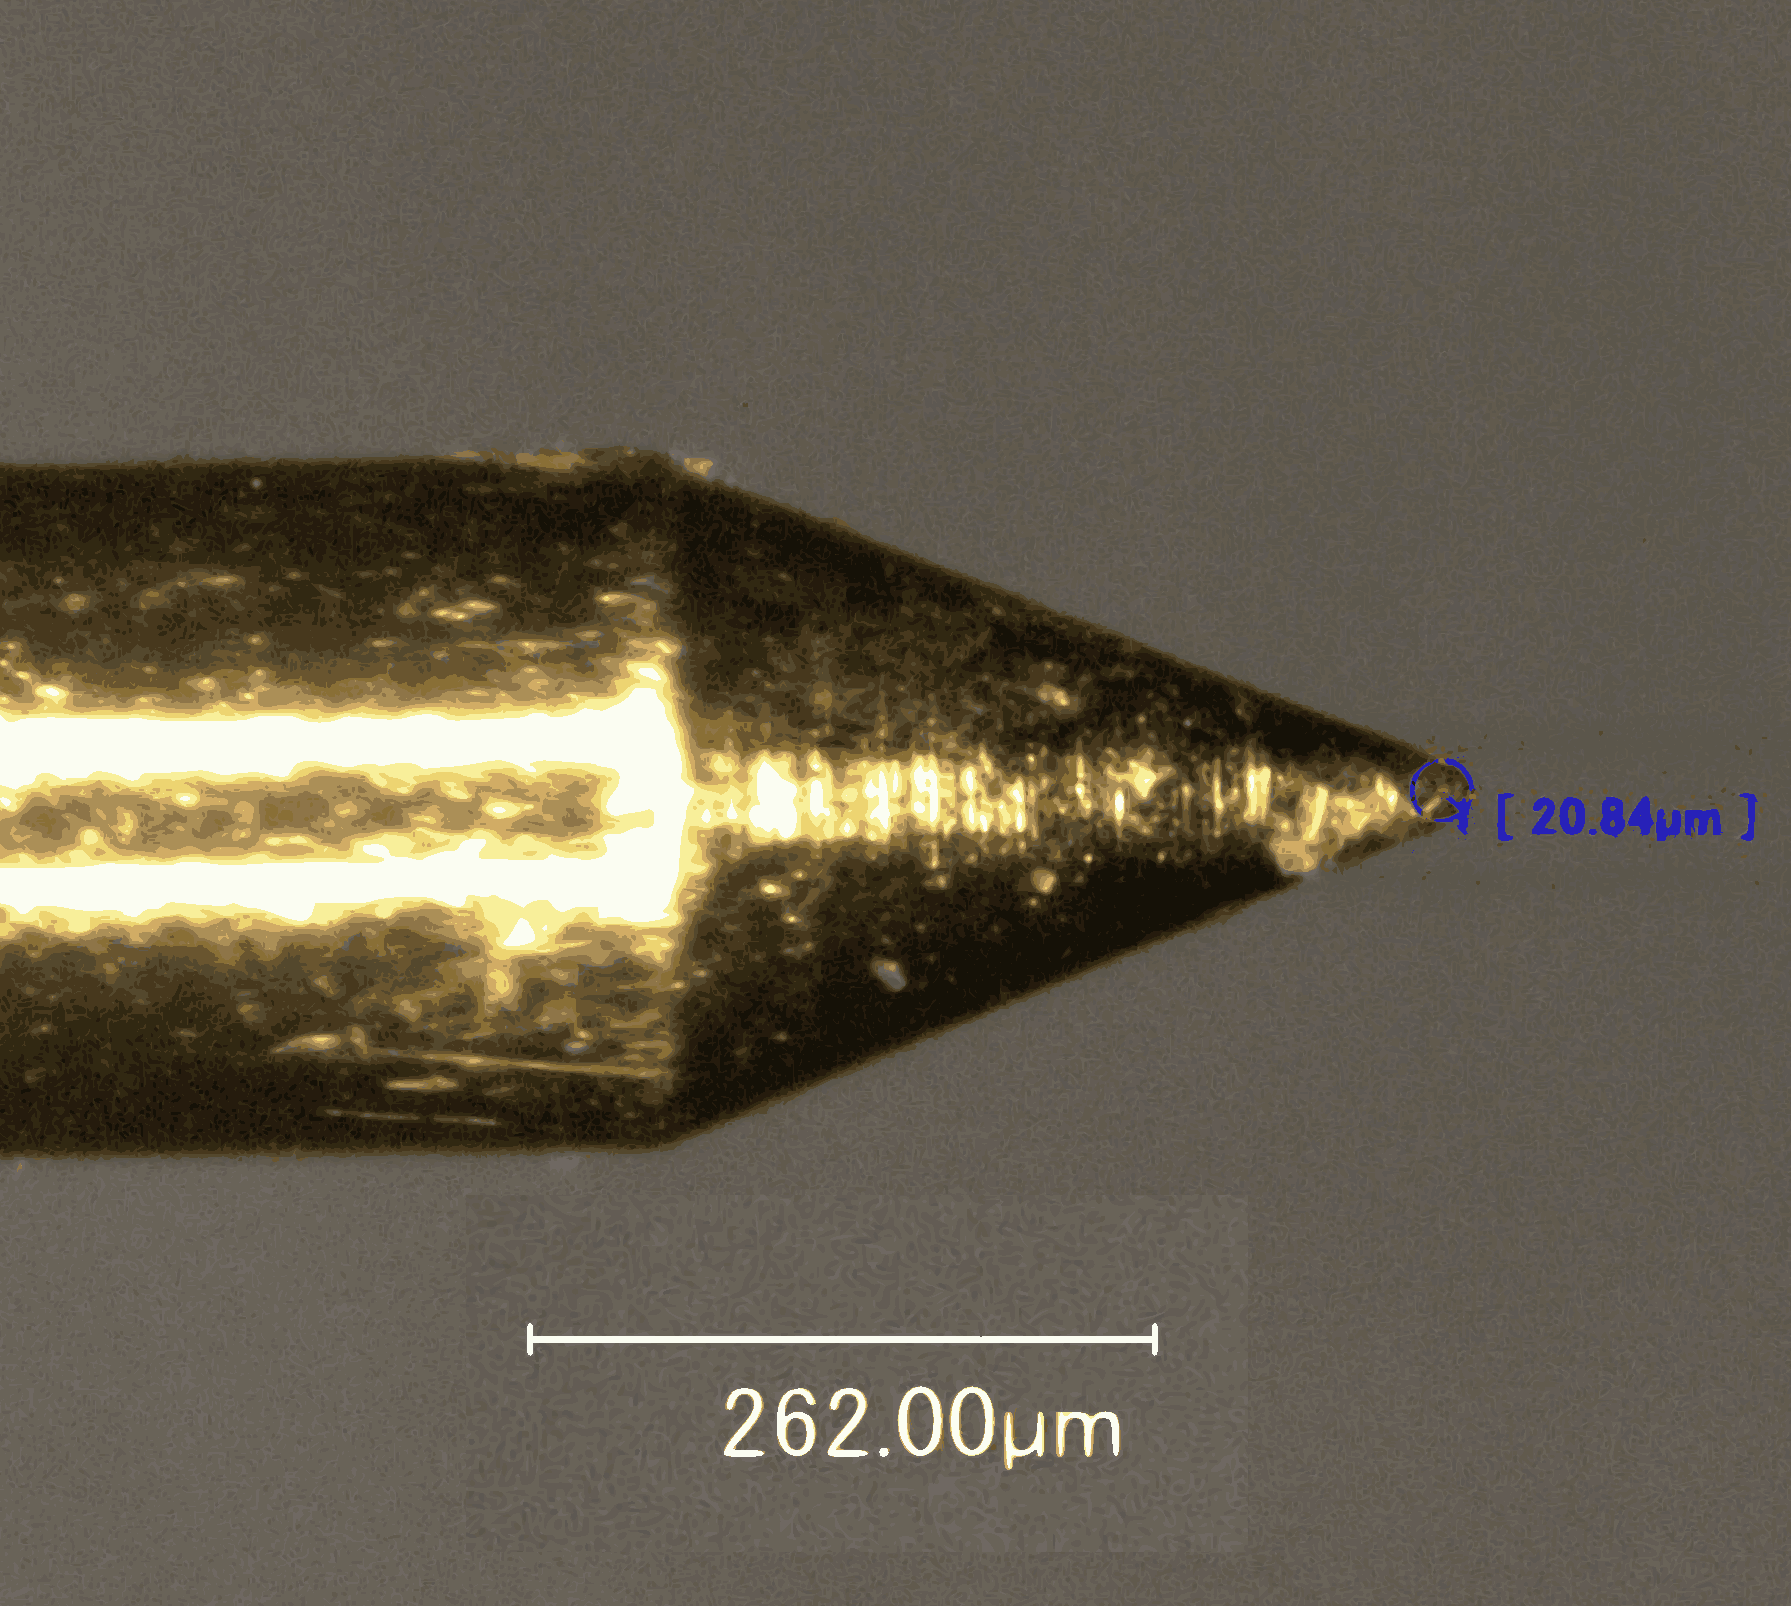
\includegraphics[width=16cm]{2_goodPractices/figures/pointeBBI.pdf}
%    \caption{BBI metallic probe measurement closer look}
%    \label{fig:pointeBBI}
%\end{figure}

\begin{figure}[ht!]
    \centering
    \begin{subfigure}[t]{7.0cm}
        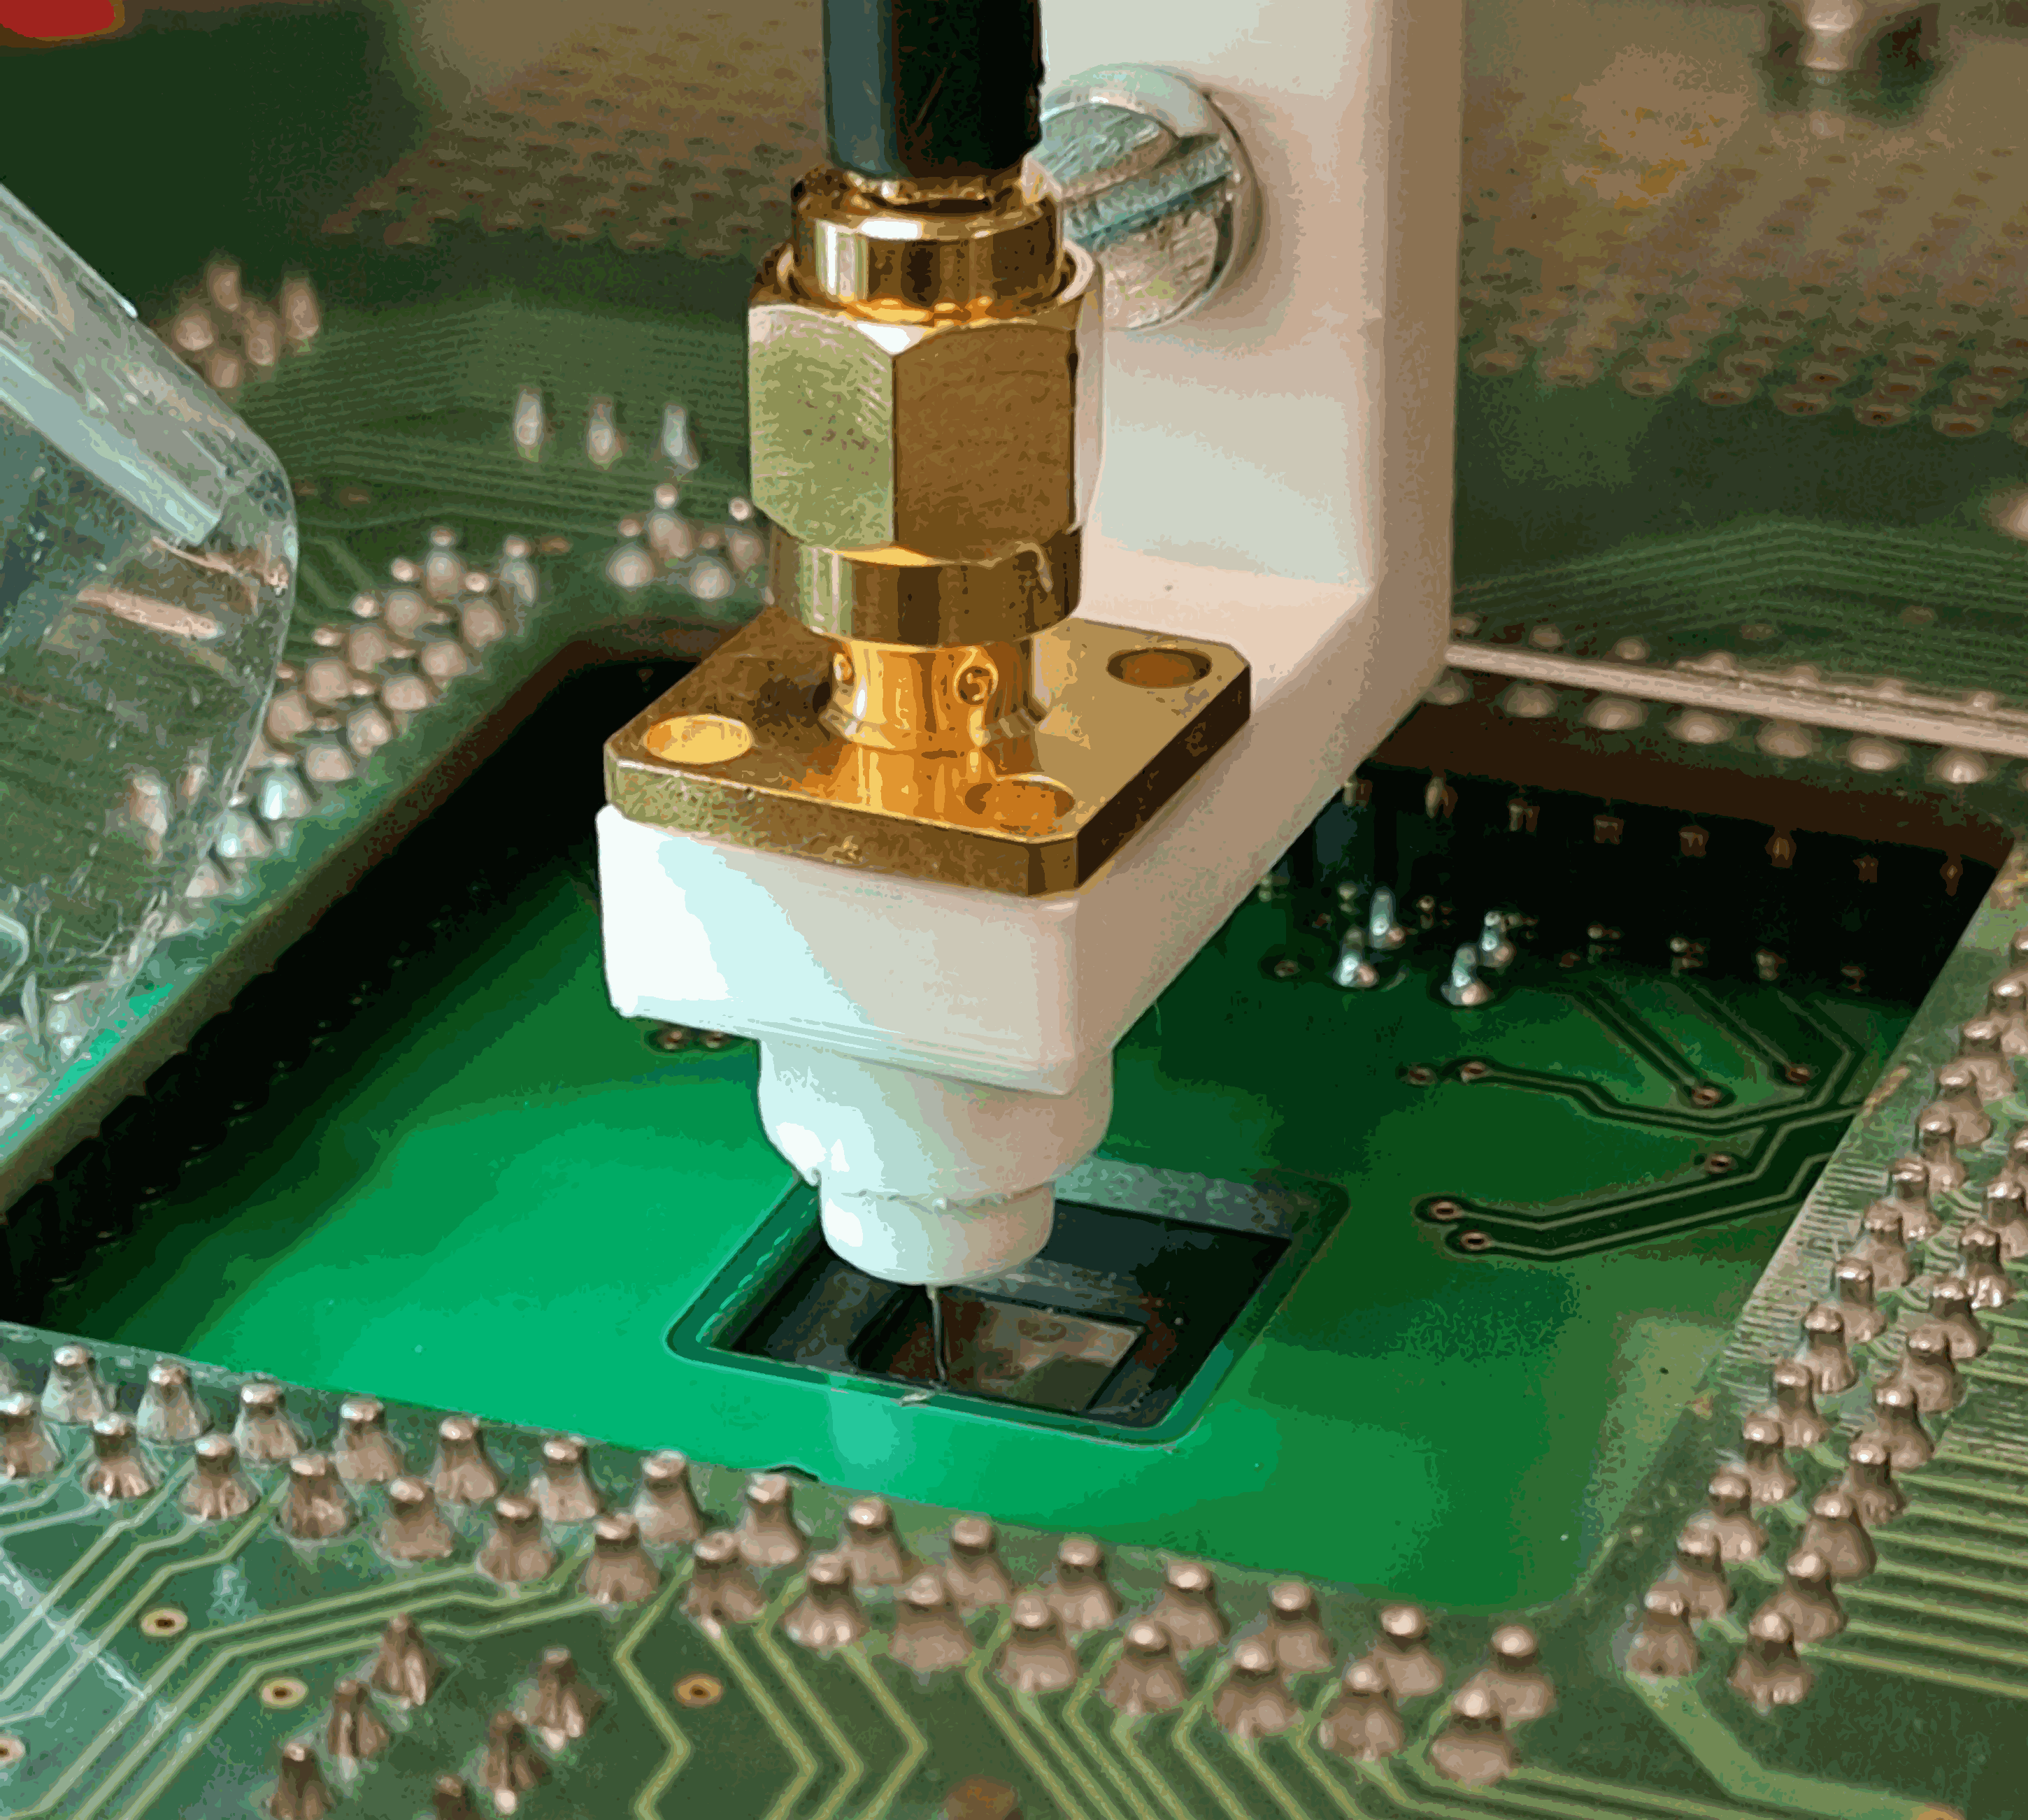
\includegraphics[height=6.8cm]{2_goodPractices/figures/sondeBBI.pdf}
        \caption{BBI metallic probe in mechanical contact with IC target}
        \label{subfig:sondeBBI}
    \end{subfigure}\hfill
    \begin{subfigure}[t]{7.0cm}
        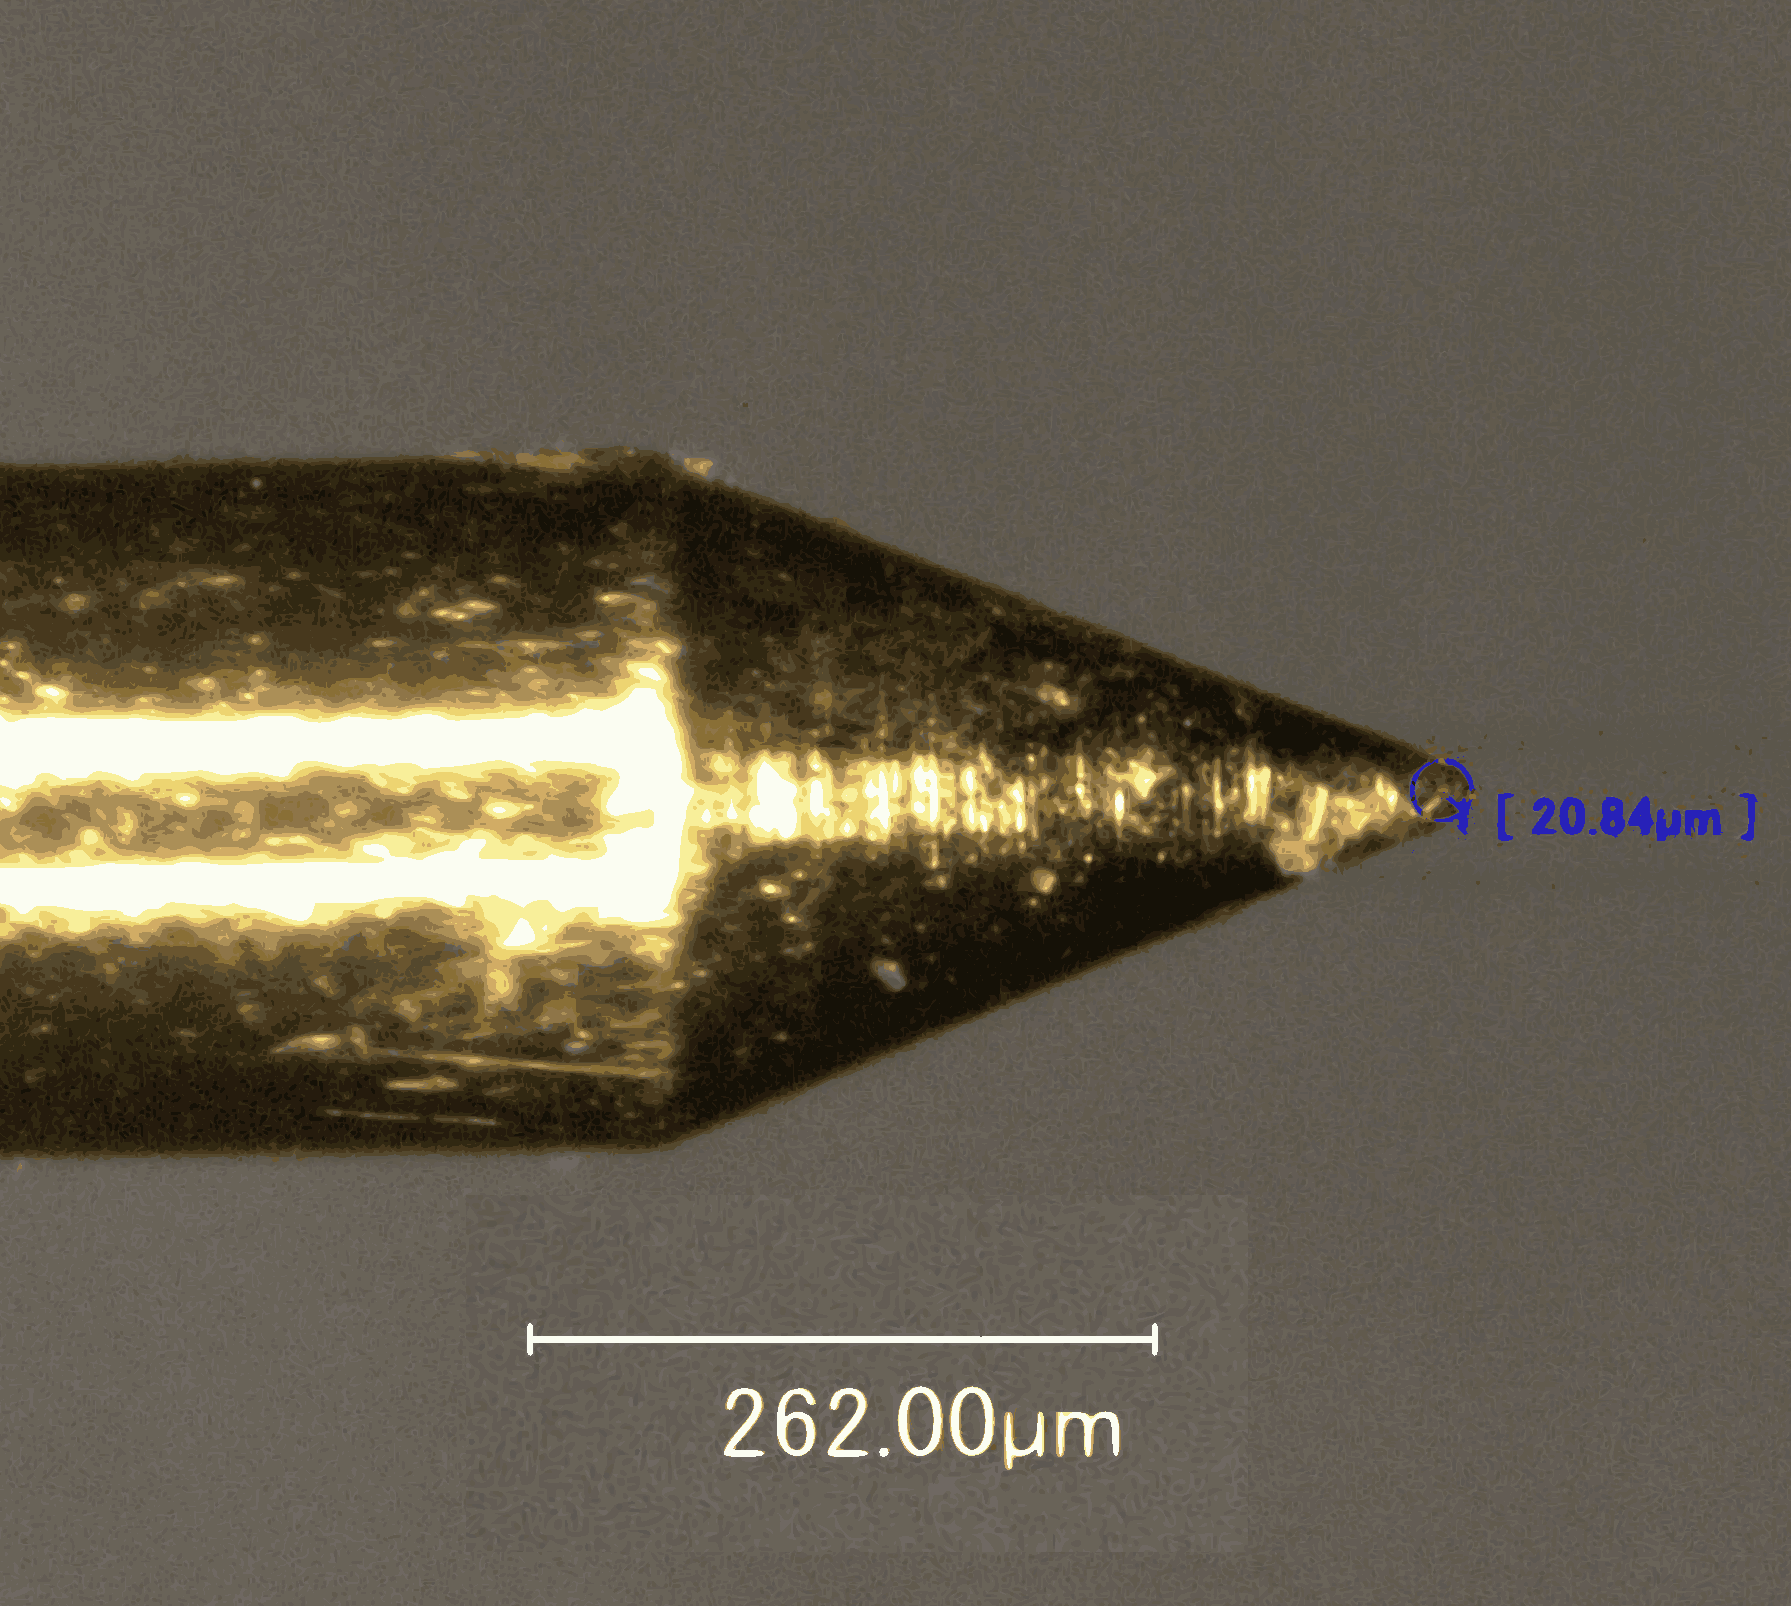
\includegraphics[height=6.8cm]{2_goodPractices/figures/pointeBBI.pdf}
        \caption{BBI metallic probe measurement closer look}
        \label{subfig:pointeBBI}
    \end{subfigure}
    \caption{Dual-well and triple-well inverter silicon sectional view.}
    \label{fig:sondePointeBBI}
\end{figure}
The most distinctive piece of equipment when working with BBI compared to other fault injection methods is the electrical probe.
It is commonly made with a metal tip, a connector of any sort and a mechanical support to hold the structure together.
Any size available on the market can be used depending on the needs.
In the case of \bbi, the probe is used to establish the electrical contact with the substrate of integrated circuits, the latter being poorly conductive, but not isolating.
For this work, we designed a custom probe, allowing us to control its characteristics, around three simple parts:
\begin{itemize}
    \setlength\itemsep{-0.1em}
    \item An SMA connector, to have a low-cost, small and standard interconnection available with almost every high-speed equipment
    \item A spring-loaded metallic tip soldered onto the SMA connector providing a better control over the applied pressure onto the backside
    \item A custom 3D-printed support holding the parts together, shaped to fit with our other tools
\end{itemize}
Fig. \ref{fig:sondePointeBBI} shows detailed pictures of the probe we designed, with a photograph in operation in Fig. \ref{subfig:sondeBBI}, and a photograph under a microscope of the probe's tip-end in Fig. \ref{subfig:pointeBBI}, allowing to measure its actual size before its first usage.
The metallic probe we had chosen has a 0.635 mm diameter and is 16.35 mm long. The specified maximum nominal current of the probe is of 1.5 A, and the electrical contact resistance measures approximately 70 m\textOmega.
The tip has a diameter roughly equal to 20 µm, and it is important to note that this value tends to increase when the probe is utilized, due to the physical contact and the pressure with the IC backside.
The bill-of-materials cost for our custom probe tool is roughly equal to 20 \$, ignoring manual labor to assemble everything together.

\subsection{Generator \ddc}
\label{chap:2_goodPractices;sect:bbiPlatforms;subsect:generator}
The other fundamental piece of equipment when practicing \bbi is the voltage pulse generator.
It is, generally, one of the most expensive platform tool, similar to \emfi.
Indeed, because \bbi relies on voltage pulses to disturb an IC, it is necessary to provide the researcher a precise control over the pulse parameters, such as the voltage set point, the pulse duration, the rise and fall times, etc.
However, these pas few years have been introduced lower cost alternatives, at the cost of some drawbacks which, in some cases, can be a good compromise between cost and accuracy.
During my work, I used a precise voltage pulse generator to be able to finely study the voltage pulse characteristics effects on \bbi, but because other alternatives exist, I introduce one of them in this section, alongside the fast and precise generator available at our laboratory.

\subsubsection{Low-cost generator \ddc}

\begin{figure}[H]
    \centering
    \includegraphics[width=\textwidth]{2_goodPractices/figures/picoemp-red.jpeg}
    \caption{ChipSHOUTER\textregistered-PicoEMP from NewAE Technology Inc.}
    \label{fig:newAeChipShouter}
\end{figure}
The low-cost generator presented in this section is the NewAE Technology Inc. ChipSHOUTER\textregistered-PicoEMP, illustrated in Fig. \ref{fig:newAeChipShouter}.
Despite being originally designed for \emfi, it is suitable as well for \bbi.
The bill-of-materials for this tool is roughly equal to 15 \$, excluding the manual labor, which is less than our custom probe.
It also has the advantage of being open-source, making it a future-proof community maintainable solution.
Its main characteristics and drawbacks are the following:
\begin{itemize}
    \setlength\itemsep{-0.1em}
    \item The output transformer is low-power, around up to 200 mW
    \item It uses a transformer, therefore no DC voltage option is available at its output
    \item The recovery time is slow, measured between 1 to 4 seconds depending on operating conditions
    \item The maximum voltage pulse is of approximately 250 V
    \item There is no pre-calibration
    \item It does not allow pulse width control by default. However, it is possible through drive signal control, even though being less accurate.
\end{itemize}

\subsubsection{Fast, high voltage generator \ddc}

\begin{figure}[H]
    \centering
    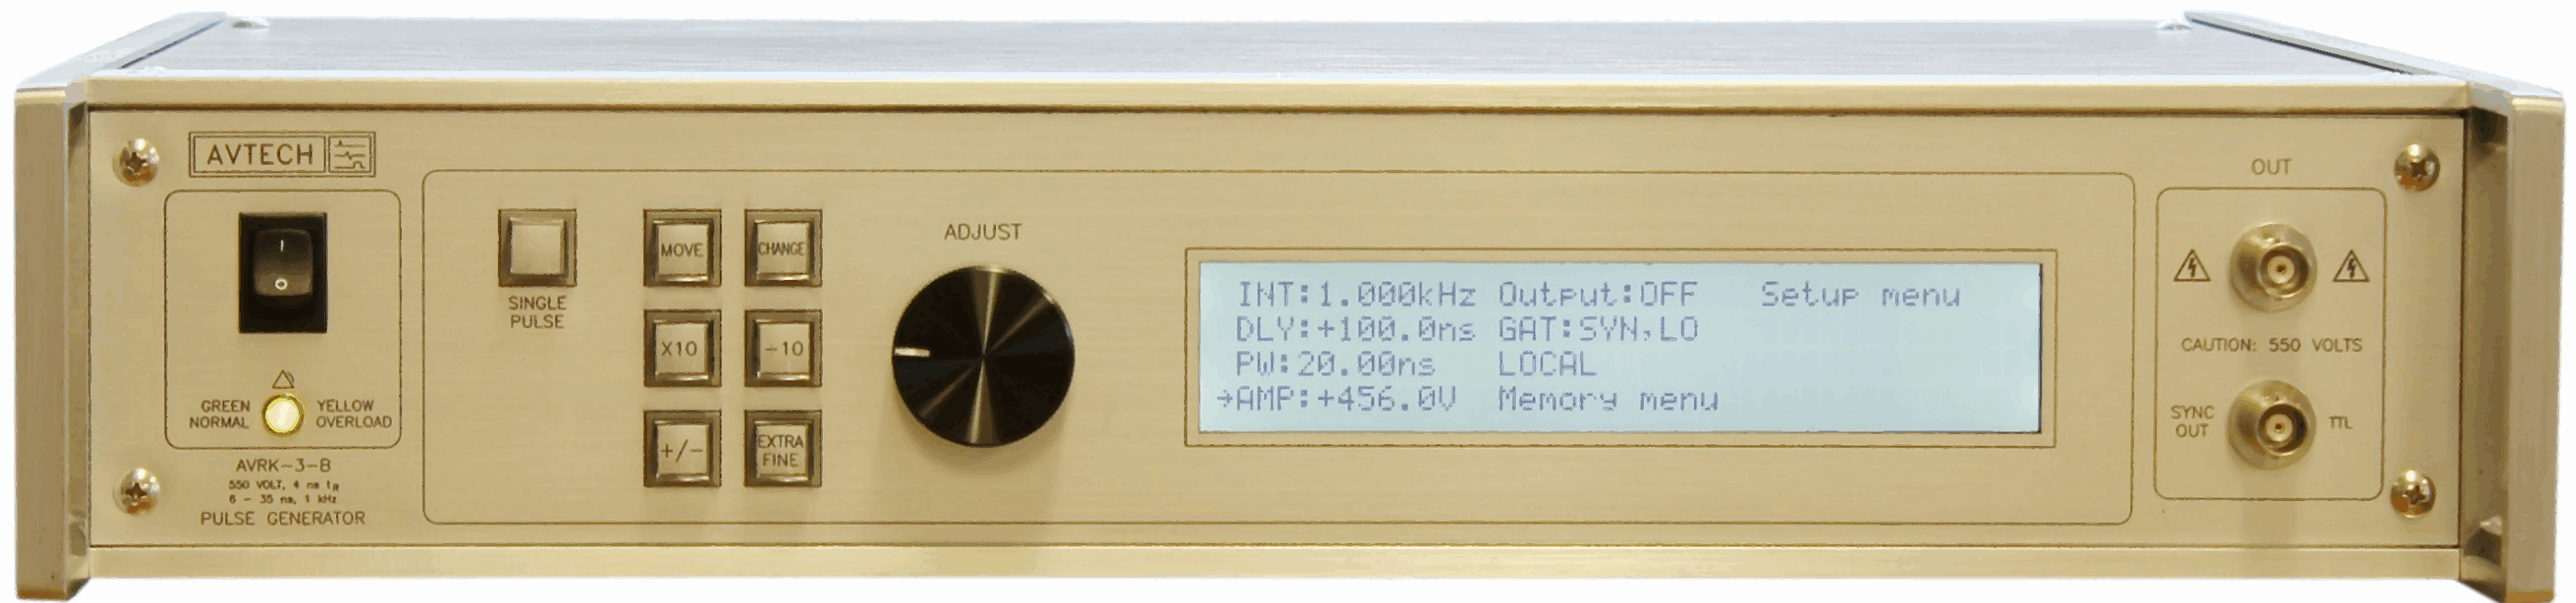
\includegraphics[width=\textwidth]{2_goodPractices/figures/avrk4b.pdf}
    \caption{Front side of the Avtech Electrosystems Ltd. AVRK-4-B High Voltage Pulser}
    \label{fig:avrk4b}
\end{figure}
For my thesis, the generator used in all experiments is from the model AVRK-4-B from Avtech Electrosystems Ltd.
It is illustrated in Fig. \ref{fig:avrk4b}.
This generator is high-speed and high-voltage.
Similar to the low-cost generator described previously, it is commonly used for \emfi, but is also suitable for \bbi.
Its main specifications are the following:
\begin{itemize}
    \setlength\itemsep{-0.1em}
    \item The voltage pulse amplitude is specified between 150 V and 750 V with positive and negative polarities. The generator can go below and above these thresholds, there is no guarantee of the set point value correctness.
    \item The pulse width is specified between 6 ns and 20 ns. Similar to the voltage, the generator can go down from 4.5 ns, up to 22 ns, but is not specified out of the default range.
    \item Rise time (resp. fall time) for positive (resp. negative) pulses is specified to be precisely of 4 ns. Fall time(resp. rise time) for positive (resp. negative) pulses is not specified and depends on the generator load characteristics.
    \item The recovery time is inferior to 1 ms, allowing a pulse repetition frequency up to 1 kHz.
    \item The propagation delay measures 150 ns.
    \item The output is DC-coupled, allowing the generator to continue providing energy to the load (if resistive or inductive) during the pulse's plateau.
    \item All the specifications presuppose that the generator is loaded with precisely \fiftyOhms{50}.
\end{itemize}
}

% PAS ENCORE RETOUCHÉ ICI - fin
